\documentclass[border=4pt]{standalone}
\usepackage[T1]{fontenc}
\usepackage{lmodern}
\usepackage{amsmath}
\usepackage{pgfplots}
\pgfplotsset{compat=1.18}
\usepgfplotslibrary{groupplots,fillbetween}
\usetikzlibrary{calc,arrows.meta}
% one colour per kind of method, the same in every figure (Okabe-Ito)
\definecolor{neur}{HTML}{D55E00}   % neurons chosen by attribution
\definecolor{dirc}{HTML}{009E73}   % directions from the weird-vs-normal contrast
\definecolor{read}{HTML}{0072B2}   % readout methods and interventions chosen from readouts
\definecolor{pers}{HTML}{CC79A7}   % Assistant Axis / persona
\definecolor{ctrl}{HTML}{8C8C8C}   % random controls
\definecolor{meas}{HTML}{E69F00}   % measured outcome
\definecolor{ink}{HTML}{222222}
\pgfplotsset{
  every axis/.append style={clip=false, font=\small, axis line style={black!55}, tick style={black!55}, tick align=outside,
    label style={font=\small}, tick label style={font=\footnotesize}, title style={font=\small, align=center}},
  grid style={black!9, line width=0.4pt},
  every axis legend/.append style={font=\footnotesize, draw=none, fill=none},
  ci/.style={/pgfplots/error bars/x dir=both, /pgfplots/error bars/x explicit, /pgfplots/error bars/error bar style={line width=0.8pt}, /pgfplots/error bars/error mark=none},
  yci/.style={/pgfplots/error bars/y dir=both, /pgfplots/error bars/y explicit, /pgfplots/error bars/error bar style={line width=0.8pt}, /pgfplots/error bars/error mark=none},
}

\begin{document}
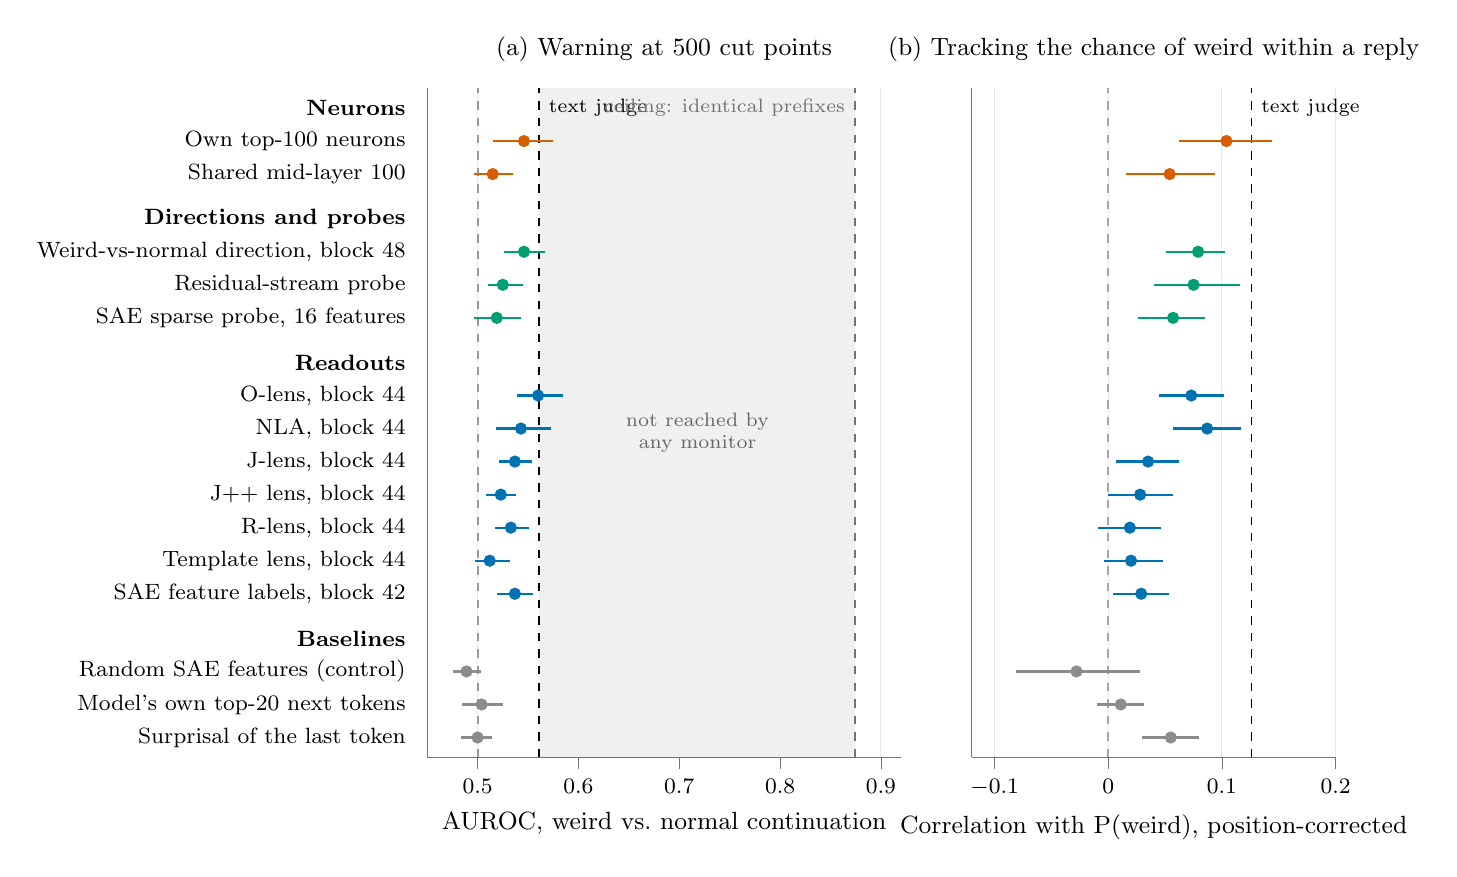
\begin{tikzpicture}
\begin{groupplot}[group style={group size=2 by 1, horizontal sep=0.9cm, y descriptions at=edge left}, height=10.08cm, ymin=-19.65, ymax=0.6, ytick={0.00,-1.00,-2.00,-3.35,-4.35,-5.35,-6.35,-7.70,-8.70,-9.70,-10.70,-11.70,-12.70,-13.70,-14.70,-16.05,-17.05,-18.05,-19.05}, yticklabels={{\textbf{Neurons}},{Own top-100 neurons},{Shared mid-layer 100},{\textbf{Directions and probes}},{Weird-vs-normal direction, block 48},{Residual-stream probe},{SAE sparse probe, 16 features},{\textbf{Readouts}},{O-lens, block 44},{NLA, block 44},{J-lens, block 44},{J++ lens, block 44},{R-lens, block 44},{Template lens, block 44},{SAE feature labels, block 42},{\textbf{Baselines}},{Random SAE features (control)},{Model's own top-20 next tokens},{Surprisal of the last token}}, y tick label style={font=\footnotesize}, major y tick style={draw=none}, axis y line*=left, axis x line*=bottom, xmajorgrids]
\nextgroupplot[width=7.6cm, xmin=0.45, xmax=0.92, xtick={0.5,0.6,0.7,0.8,0.9}, xlabel={AUROC, weird vs.\ normal continuation}, title={(a) Warning at 500 cut points}]
\fill[black!6] (axis cs:0.561,-19.65) rectangle (axis cs:0.874,0.6);
\node[font=\scriptsize, black!60, align=center] at (axis cs:0.718,-9.83) {not reached by\\any monitor};
\draw[black!40, dashed, line width=0.7pt] (axis cs:0.500,-19.65) -- (axis cs:0.500,0.6);
\draw[black, dashed, line width=0.7pt] (axis cs:0.561,-19.65) -- (axis cs:0.561,0.6);
\node[black, font=\scriptsize, anchor=west] at (axis cs:0.561,0) {text judge};
\draw[black!55, dashed, line width=0.7pt] (axis cs:0.874,-19.65) -- (axis cs:0.874,0.6);
\node[black!55, font=\scriptsize, anchor=east] at (axis cs:0.874,0) {ceiling: identical prefixes};
\addplot[only marks, mark=*, mark size=2pt, neur, ci] coordinates {(0.546,-1.00) += (0.029,0) -= (0.031,0)};
\addplot[only marks, mark=*, mark size=2pt, neur, ci] coordinates {(0.515,-2.00) += (0.020,0) -= (0.019,0)};
\addplot[only marks, mark=*, mark size=2pt, dirc, ci] coordinates {(0.546,-4.35) += (0.021,0) -= (0.020,0)};
\addplot[only marks, mark=*, mark size=2pt, dirc, ci] coordinates {(0.525,-5.35) += (0.020,0) -= (0.015,0)};
\addplot[only marks, mark=*, mark size=2pt, dirc, ci] coordinates {(0.519,-6.35) += (0.024,0) -= (0.023,0)};
\addplot[only marks, mark=*, mark size=2pt, read, ci] coordinates {(0.560,-8.70) += (0.025,0) -= (0.021,0)};
\addplot[only marks, mark=*, mark size=2pt, read, ci] coordinates {(0.543,-9.70) += (0.030,0) -= (0.025,0)};
\addplot[only marks, mark=*, mark size=2pt, read, ci] coordinates {(0.537,-10.70) += (0.017,0) -= (0.016,0)};
\addplot[only marks, mark=*, mark size=2pt, read, ci] coordinates {(0.523,-11.70) += (0.015,0) -= (0.015,0)};
\addplot[only marks, mark=*, mark size=2pt, read, ci] coordinates {(0.533,-12.70) += (0.018,0) -= (0.016,0)};
\addplot[only marks, mark=*, mark size=2pt, read, ci] coordinates {(0.512,-13.70) += (0.020,0) -= (0.015,0)};
\addplot[only marks, mark=*, mark size=2pt, read, ci] coordinates {(0.537,-14.70) += (0.018,0) -= (0.018,0)};
\addplot[only marks, mark=*, mark size=2pt, ctrl, ci] coordinates {(0.489,-17.05) += (0.014,0) -= (0.013,0)};
\addplot[only marks, mark=*, mark size=2pt, ctrl, ci] coordinates {(0.504,-18.05) += (0.021,0) -= (0.019,0)};
\addplot[only marks, mark=*, mark size=2pt, ctrl, ci] coordinates {(0.500,-19.05) += (0.014,0) -= (0.016,0)};
\nextgroupplot[width=6.2cm, xmin=-0.12, xmax=0.2, xtick={-0.1,0,0.1,0.2}, scaled x ticks=false, xticklabel style={/pgf/number format/.cd, fixed, precision=1}, xlabel={Correlation with P(weird), position-corrected}, title={(b) Tracking the chance of weird within a reply}]
\draw[black!35, dashed, line width=0.7pt] (axis cs:0,-19.65) -- (axis cs:0,0.6);
\draw[black, dashed, line width=0.7pt] (axis cs:0.126,-19.65) -- (axis cs:0.126,0.6);
\node[font=\scriptsize, anchor=west] at (axis cs:0.126,0) {text judge};
\addplot[only marks, mark=*, mark size=2pt, neur, ci] coordinates {(0.104,-1.00) += (0.040,0) -= (0.042,0)};
\addplot[only marks, mark=*, mark size=2pt, neur, ci] coordinates {(0.054,-2.00) += (0.040,0) -= (0.038,0)};
\addplot[only marks, mark=*, mark size=2pt, dirc, ci] coordinates {(0.079,-4.35) += (0.024,0) -= (0.028,0)};
\addplot[only marks, mark=*, mark size=2pt, dirc, ci] coordinates {(0.075,-5.35) += (0.041,0) -= (0.035,0)};
\addplot[only marks, mark=*, mark size=2pt, dirc, ci] coordinates {(0.057,-6.35) += (0.028,0) -= (0.031,0)};
\addplot[only marks, mark=*, mark size=2pt, read, ci] coordinates {(0.073,-8.70) += (0.029,0) -= (0.028,0)};
\addplot[only marks, mark=*, mark size=2pt, read, ci] coordinates {(0.087,-9.70) += (0.030,0) -= (0.030,0)};
\addplot[only marks, mark=*, mark size=2pt, read, ci] coordinates {(0.035,-10.70) += (0.027,0) -= (0.028,0)};
\addplot[only marks, mark=*, mark size=2pt, read, ci] coordinates {(0.028,-11.70) += (0.029,0) -= (0.028,0)};
\addplot[only marks, mark=*, mark size=2pt, read, ci] coordinates {(0.019,-12.70) += (0.027,0) -= (0.028,0)};
\addplot[only marks, mark=*, mark size=2pt, read, ci] coordinates {(0.020,-13.70) += (0.028,0) -= (0.024,0)};
\addplot[only marks, mark=*, mark size=2pt, read, ci] coordinates {(0.029,-14.70) += (0.024,0) -= (0.025,0)};
\addplot[only marks, mark=*, mark size=2pt, ctrl, ci] coordinates {(-0.028,-17.05) += (0.056,0) -= (0.053,0)};
\addplot[only marks, mark=*, mark size=2pt, ctrl, ci] coordinates {(0.011,-18.05) += (0.020,0) -= (0.021,0)};
\addplot[only marks, mark=*, mark size=2pt, ctrl, ci] coordinates {(0.055,-19.05) += (0.025,0) -= (0.025,0)};
\end{groupplot}
\end{tikzpicture}
\end{document}
